\documentclass[compress]{beamer}
\usepackage{ifthen,verbatim}

\newcommand{\isnote}{}
\xdefinecolor{lightyellow}{rgb}{1.,1.,0.25}
\xdefinecolor{darkblue}{rgb}{0.1,0.1,0.7}
\xdefinecolor{purple}{rgb}{0.5,0.1,0.7}

%% Uncomment this to get annotations
%% \def\notes{\addtocounter{page}{-1}
%%            \renewcommand{\isnote}{*}
%% 	   \beamertemplateshadingbackground{lightyellow}{white}
%%            \begin{frame}
%%            \frametitle{Notes for the previous page (page \insertpagenumber)}
%%            \itemize}
%% \def\endnotes{\enditemize
%% 	      \end{frame}
%%               \beamertemplateshadingbackground{white}{white}
%%               \renewcommand{\isnote}{}}

%% Uncomment this to not get annotations
\def\notes{\comment}
\def\endnotes{\endcomment}

\setbeamertemplate{navigation symbols}{}
\setbeamertemplate{headline}{\mbox{ } \hfill
\begin{minipage}{5.5 cm}
\vspace{-0.75 cm} \small
\end{minipage} \hfill
\begin{minipage}{4.5 cm}
\vspace{-0.75 cm} \small
\begin{flushright}
\ifthenelse{\equal{\insertpagenumber}{1}}{}{Jim Pivarski \hspace{0.2 cm} \insertpagenumber\isnote/\pageref{numpages}}
\end{flushright}
\end{minipage}\mbox{\hspace{0.2 cm}}\includegraphics[height=1 cm]{../cmslogo} \hspace{0.1 cm} \includegraphics[height=1 cm]{../tamulogo} \hspace{0.01 cm} \vspace{-1.05 cm}}

\begin{document}
\begin{frame}
\vfill
\begin{center}
\textcolor{darkblue}{\Large Muon Wheel/Disk Alignment Constants from HIP}

\vfill
\begin{columns}
\column{0.3\linewidth}
\begin{center}
\large
\textcolor{darkblue}{Jim Pivarski}

\vspace{0.2 cm}
Alexei Safonov

\vspace{0.2 cm}
Sergey Senkin
\end{center}

\column{0.3\linewidth}
\begin{center}
\large
K\'aroly Banicz
\end{center}
\end{columns}

\begin{columns}
\column{0.3\linewidth}
\begin{center}
\scriptsize
{\it Texas A\&M University}
\end{center}
\column{0.3\linewidth}
\begin{center}
\scriptsize
{\it US-CMS}
\end{center}
\end{columns}

\vfill
12 November, 2008

\end{center}
\end{frame}

%% \begin{notes}
%% \item This is the annotated version of my talk.
%% \item If you want the version that I am presenting, download the one
%% labeled ``slides'' on Indico (or just ignore these yellow pages).
%% \item The annotated version is provided for extra detail and a written
%% record of comments that I intend to make orally.
%% \item Yellow notes refer to the content on the {\it previous} page.
%% \item All other slides are identical for the two versions.
%% \end{notes}

\small

\begin{frame}
\frametitle{Outline}
\begin{itemize}
\item Reminder of method
\item Alignment results
\end{itemize}

\vspace{-1.5 cm}
\mbox{ } \hfill 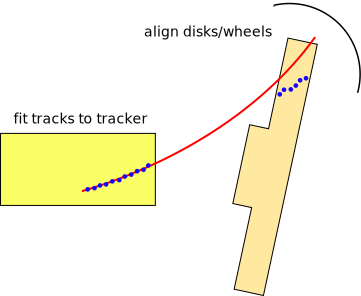
\includegraphics[width=0.4\linewidth]{globalMuon_alignment.png}

\vspace{-0.75 cm}
\hspace{-0.83 cm} \textcolor{darkblue}{\Large Reminder of method}

\vspace{0.25 cm}
\begin{itemize}
\item Treat 5 barrel wheels and 6 out of 8 endcap disks as 6-dof \mbox{rigid bodies\hspace{-1 cm}}
\item Select CRAFT global cosmic rays passing through tracker and wheel/disk
\item Fit tracker part, propagate to wheel/disk, align wheel/disk
\begin{itemize}
\item ME$\pm$4/1 and inner rings (ME$\pm$1/1, 2/1, 3/1) are nearly
  inaccessible (dozens of poor-quality tracks)
\item track-fitting and alignment step are independent, they do not require iteration to resolve any correlation between them
\end{itemize}
\item Every track residual can be converted into 6-dof \mbox{alignment corrections\hspace{-1 cm}}
\end{itemize}

\end{frame}

%% \section*{First section}
%% \begin{frame}
%% \begin{center}
%% \Huge \textcolor{blue}{First section}
%% \end{center}
%% \end{frame}


\begin{frame}
\frametitle{Selecting tracks by $p_T$}

\begin{columns}
\column{0.6\linewidth}

\begin{itemize}
\item CRAFT offers new ability to reject low-momentum tracks
\item Observe each alignment parameter as a function of curvature ($q/p_T$)
\item Cleanest measurement is \mbox{above 20~GeV\hspace{-1 cm}}
\end{itemize}

\begin{center}
\includegraphics[width=0.75\linewidth]{measurement_from_each_track.pdf}
\end{center}

\column{0.4\linewidth}
\includegraphics[height=\linewidth, angle=90]{qoverpt.pdf}

\vfill
\includegraphics[width=\linewidth]{extrapolation_to_infinite_momentum.pdf}
\end{columns}
\end{frame}

\begin{frame}
\frametitle{$p \to \infty$ extrapolation}

\begin{itemize}
\item Multiple scattering and $\vec{B}$ errors limit to zero at infinite momentum
\begin{itemize}
\item multiple scattering is symmetric (independent of $q$)
\item $\vec{B}$ errors are antisymmetric with $q$
\item both depend on track angles and detailed track distribution
\end{itemize}

\item Taylor-expand around $q/p_T = 0$ up to second order
\item \textcolor{darkblue}{Constant term ($p_0$) is the misalignment: alignment minimizes $p_0$}
\item Linear term ($p_1$) is $\vec{B}$ error, sensitive to $\pm$0.0007-0.02~T (dep.\ on $\eta$)
\end{itemize}

\begin{columns}
\column{0.33\linewidth}
\mbox{ } \hfill ME$+$2 $z$ \hfill \mbox{ }

\vspace{0.1 cm}
\includegraphics[width=\linewidth]{extrapolation_to_infinite_momentum.pdf}
\column{0.33\linewidth}
\mbox{ } \hfill Wheel 0 $z$ \hfill \mbox{ }

\vspace{0.1 cm}
\includegraphics[width=\linewidth]{extrapolation_wheel0.pdf}
\column{0.33\linewidth}
\mbox{ } \hfill ME$+$2 $\phi_z$ \hfill \mbox{ }

\vspace{0.1 cm}
\includegraphics[width=\linewidth]{extrapolation_phiz.pdf}
\end{columns}
\end{frame}

\begin{frame}
\frametitle{Details}
\begin{itemize}\setlength{\itemsep}{0.3 cm}
\item Barrel and endcap are treated equally

\item Hits in the same chamber/superlayer on the same track are
  combined, so that profile-plot error bars are meaningful:
  fit-uncertainty in $p_0$ is the alignment uncertainty

\item Wheels internally maintain the relative alignment of chambers

\item Disks are aligned with tracks passing through outer ring only
  (allows them to maintain inner ring correction from \mbox{hardware measurement)\hspace{-1 cm}}

\item Quality cuts: tracker $\chi^2/N_{\mbox{\scriptsize dof}} < 20$,
  $N_{\mbox{\scriptsize tracker hits}} \ge 10$, at least 500 tracks
  per alignable

\item Iterate to verify residual $\to$ 0

\end{itemize}
\end{frame}

\begin{frame}
\frametitle{All alignment results (\only<1>{1}\only<2>{2}\only<3>{3}\only<4>{4}\only<5>{5}\only<6>{6}/6)}

\vfill
\begin{itemize}
\item Four run regions with stable 3.8~T field
\item Results depend on tracker alignment: this uses last night's final tracker alignment (HIP with survey constraints)
\item \only<1>{Aligned CMS is {\it compressed} in $z$}\only<2>{$\phi_z$ is the rotation relative to tracker: essential for charge ratio}\only<3>{$x$ (horizontal) corrections}\only<4>{$\phi_x$ rotation around the $x$ axis, essentially a $z$ difference between top and bottom}\only<5>{$y$ is poorly determined by vertical cosmic rays, we weighted the profile plots to prefer tracks with good measurements}\only<6>{same for $\phi_y$ (best determined by non-vertical tracks), also weighted}
\end{itemize}

\vfill
\only<1>{\includegraphics[height=\linewidth, angle=90]{alierr_z.pdf}}
\only<2>{\includegraphics[height=\linewidth, angle=90]{alierr_phiz.pdf}}
\only<3>{\includegraphics[height=\linewidth, angle=90]{alierr_x.pdf}}
\only<4>{\includegraphics[height=\linewidth, angle=90]{alierr_phix.pdf}}
\only<5>{\includegraphics[height=\linewidth, angle=90]{alierr_y.pdf}}
\only<6>{\includegraphics[height=\linewidth, angle=90]{alierr_phiy.pdf}}

%% \only<1>{\includegraphics[height=\linewidth, angle=90]{bydataset_final_z.pdf}}
%% \only<2>{\includegraphics[height=\linewidth, angle=90]{bydataset_final_phiz.pdf}}
%% \only<3>{\includegraphics[height=\linewidth, angle=90]{bydataset_final_x.pdf}}
%% \only<4>{\includegraphics[height=\linewidth, angle=90]{bydataset_final_y.pdf}}
%% \only<5>{\includegraphics[height=\linewidth, angle=90]{bydataset_final_phix.pdf}}
%% \only<6>{\includegraphics[height=\linewidth, angle=90]{bydataset_final_phiy.pdf}}
\end{frame}

\begin{frame}
\frametitle{Conclusions}
\begin{itemize}\setlength{\itemsep}{0.25 cm}
\item Ideal wheel/disk positions (no correction) are known to be wrong
  by millimeters or milliradians; these corrections are {\it at least} a
  step in the right direction
\item $p\to\infty$ fit emphasizes the highest $p_T$ tracks and removes
  sensitivity to multiple scattering and $\vec{B}$ field errors
\item Consistent run-by-run (different $\vec{B}$ field ramp-up periods)
\item There seems to be a good correlation between the two algorithms,
  HIP and MillePede (we should overlay them, once new tracker
  alignment is incorporated)
\item $\phi_z$ is especially important for charge ratio; getting these
  constants in the first CRAFT re-processing (with refinements later)
  will help this analysis to move forward before the second re-processing
\end{itemize}
\label{numpages}
\end{frame}

\end{document}
